\subsection{Problems}

\noindent {\bf Problem \thesection.\theprob}\stepcounter{prob}

The input mechanical power of a water pump is 25 kW, the revolution number is 1440 rpm, the flow rate is 0.06 $\mathrm{m^3/s}$. The volumetric efficiency is estimated as $\eta_v=0.92$, the hydraulic efficiency is $\eta_h=0.85$, the disc friction power loss is $P'_{df}=0.9$ kW, the mechanical loss is $P'_m=1.3$ kW. Find the head and the specific speed and make a sketch of the impeller. (Solution: H=30.3m, $n_q$=27.3, the impeller is a thin radial one.)

%%%%%%%%%%%%%%%%%%%%%%%%%%%%%%%%%%%%%%%%%%%%%%%%%%%%%%%%%%%%%%%%%%%%

\vspace{1cm}
\noindent {\bf Problem \thesection.\theprob}\stepcounter{prob}

The revolution number of a pump is 1450 rpm, the head and flow rate at the best-efficiency point are 17m and 0.03 $\mathrm{m^3/s}$. Find the specific speed. Find the diameter of the impeller if, based on industrial experience, the pressure number at the best-efficiency point should be $\psi=1$. Find the flow number $\varphi$. Find the head and flow rate at 970rpm. (Solution: $n_q=30$, $D_2=240$mm, $\varphi=0.036$, $Q_{970\mathrm{rpm}}=0.02\mathrm{m^3/s}$, $H_{970\mathrm{rpm}}=7.61\mathrm{m}$) 

%%%%%%%%%%%%%%%%%%%%%%%%%%%%%%%%%%%%%%%%%%%%%%%%%%%%%%%%%%%%%%%%%

\vspace{1cm}
\noindent {\bf Problem \thesection.\theprob}\stepcounter{prob}

The head produced by a six stage pump type CR 8-60 is $H[m] = 68-0.2Q^2$, the speed of rotation is $n=2850~\frac{1}{\mathrm{min}}$. The efficiency is $\eta = 0.66-0.00731 (Q-9.5)^2$. The unit of the flow rate in the formulae is $[m3/h]$. Find the specific speed. Based on the specific speed, find the type of the impeller. Determine the input power of the water delivering pump for zero delivery $Q=0$ by extrapolation from calculated points in the range $Q = 1.5; 1; 0.5 m3/h$, and using L'Hopital's rule. (Solution: $n_q=29.9$, hence the impeller is radial; $P_{in}=1334W$.)

%%%%%%%%%%%%%%%%%%%%%%%%%%%%%%%%%%%%%%%%%%%%%%%%%%%%%%%%%%%%%%%%%

\vspace{1cm}
\begin{tcolorbox}
\noindent {\bf Problem \thesection.\theprob}\stepcounter{prob}

The characteristic curve of a pump at $n_1 = 1450/min$ rotor speed is $H_1 = 40m-40000s^2/m^5 Q^2$. Calculate 5 points of the pump-characteristic for the rotor speed $n_2 = 2900/min$ in the flow rate range $Q_2 = 0,01m^3/s-0,05m^3/s$ at $0,01 m^3/s$ intervals. According to laboratory tests the affinity law is valid in this range. Give the equation of the characteristics $H_2(Q_2)$ for the rotor speed $n_2$! (Solution: $H_2(Q_2)=160-40000Q_{2}^{2}$)
\vspace{0.2cm}

Solution:
\vspace{0.2cm}

{\bf Affinity laws:}

\begin{equation*}
	\frac{q_2}{q1}=\frac{n_2}{n_1}=2, \quad
	\frac{H_2}{H_1}=\left(\frac{n_2}{n_1}\right)^2=2^2=4
	\quad \text{and} \quad \frac{P_2}{P_1}=\left(\frac{n_2}{n1}\right)^3=2^3=8.
\end{equation*}
\vspace{0.2cm}

\begin{center}
\begin{tabular}{|c|c|c|c|c|c|c|c|}
	\hline
2.with affinity & $q_1 =q_2/2[m^3/s]$ & 0 & 0.005 & 0.01 & 0.015 & 0.02  & 0.025 \\
	\hline
3.with the caracteristic curve	& $H_1$[m] & 40 & 39 & 36 & 31 & 24 & 15 \\
	\hline
1.given & $q_2$ $[m^3/s]$ & 0 & 0.01 & 0.02 & 0.03 & 0.04 & 0.05 \\
	\hline
4.with affinity	& $H_2=4H_1$ & 160 & 156 & 144 & 124 & 96 & 60 \\
	\hline
\end{tabular}
\end{center}

\vspace{0.2cm}

{\bf Conversion of the characteristic curve analytically}

the general shape of the characteristic curve of a pump at n1 speed: $H_1=A+Bq+Cq^2$ (n this case we assumed that the characteristic curve H(q) of a pump can be described with a second degree polynomial. In reality this is a good approximation). In the present problem, the linear term (Bq) is zero.

\begin{equation*}
	H_1=A+Bq+C^2q=A+C^2q.
\end{equation*}
%(Of course, if in another task, in the case of another pump, B $\ne$ 0, the following derivation can also be performed)
%Derivation:
%
We have:
%
\begin{equation*}
	H_2=H_1\left(\frac{n_2}{n_1}\right)^2=\left(\frac{n_2}{n_1}\right)^2\left(A+C{q_1}^2\right)=1\left(\frac{n_2}{n_1}\right)^2\left[A+C{q_2}^2\left(\frac{n_1}{n_2}\right)^2\right]=A\left(\frac{n_2}{n_1}\right)^2+C{q_2}^2.
\end{equation*}
In the first step of the above derivation, the affinity for the transport height H is used, in the second the characteristic curve $H_1$ is substituted. In the third we also use the affinity for the volume flows rate q, and in the fourth we remove the parantheses from the equation. The caracteristic curve of the pump is:
%
\begin{equation*}
	H_2=A\left(\frac{n_2}{n_1}\right)^2+Cq^2=40\times\left(\frac{2920}{1460}\right)^2-40000q^2.
\end{equation*}

If the linear term $B$ is non-zero, we have
%
\begin{equation*}
	H_2=A\left(\frac{n_2}{n_1}\right)^2+B\left(\frac{n_2}{n_1}\right)q_2+C{q_2}^2.
\end{equation*}

The specific speed is
%
\begin{equation*}
	n_q=n_2 {q_{2,opt}}^{1/2}{H_{2,opt}}^{-3/4}=2920\times\frac{\sqrt{0.03}}{{124}^{3/4}}=43.04.
\end{equation*}
%
Note that this number is independent of the actual revolution number (as long as the optimal head and flow rate is properly used), which justifies its name. Finally, the characteristic curves are plotted in Figure \ref{gen_fig}

\end{tcolorbox}

\begin{figure}[ht]
\begin{center}
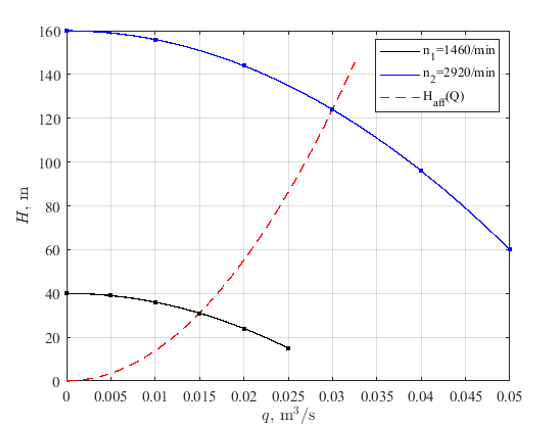
\includegraphics[scale=0.75]{figs/problem_2p4p22_aff_fig.png}
\caption{\label{gen_fig}Convert characteristic curves to other speeds}
\end{center}
\end{figure}

\vspace{1cm}

\noindent {\bf Problem \thesection.\theprob}%\stepcounter{prob} NEM ITT, AZ ABRA UTAN

Find the specific speed of the pump given by \ref{fig:PS_PerfCurves}, if the revolution number is 3000 rpm. Make a sketch of the impeller. (Solution: $n_q=92$, mixed impeller.)

\begin{figure}[!h]
\begin{center}
\centering
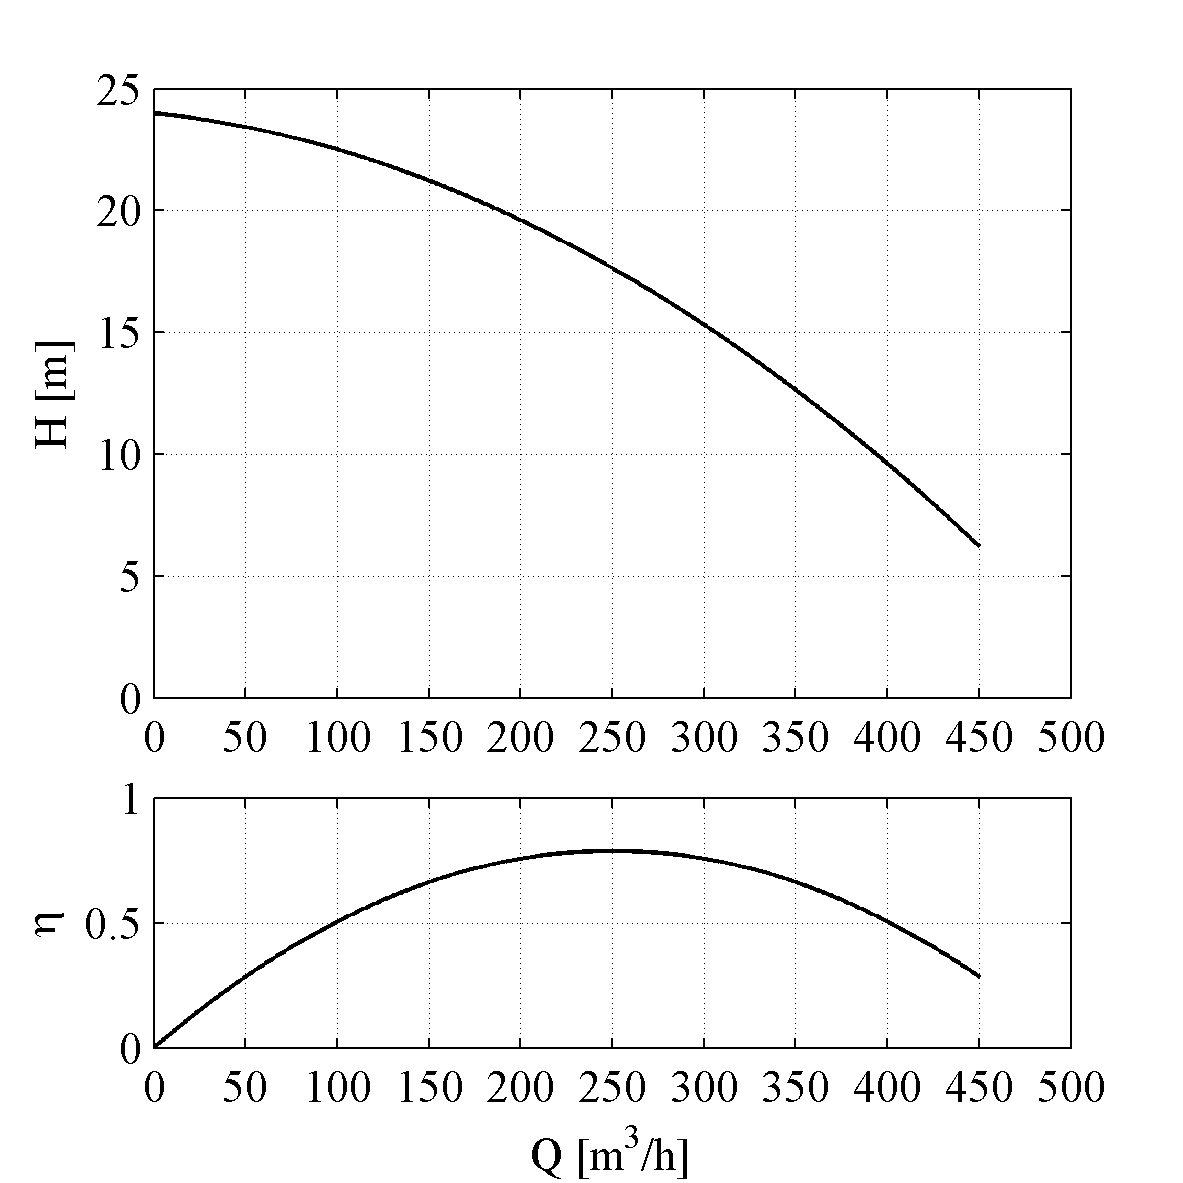
\includegraphics{Problem_solving/figs/PS_PerfCurves.png}
\caption{\label{fig:PS_PerfCurves}Performance chart for Problem \thesection.\theprob.}
\end{center}
\end{figure}
\stepcounter{prob}

%%%%%%%%%%%%%%%%%%%%%%%%%%%%%%%%%%%%%%%%%%%%%
\vspace{1cm}
\noindent {\bf Problem \thesection.\theprob}\stepcounter{prob}

The performance curve of a pump at 1450 rpm is given by $H=100-30000\,Q^2$ and the efficiency is given by $\eta=-78000\,Q^2+4500\,Q$. Find the head and flow rate of the best-efficiency point. Find the performance curve at 1740 rpm. ($H_{opt}=76$m, $Q_{opt}=0.02855\mathrm{m^3/s}$, $\eta_{max}=64.9\%$, $H_{1740\mathrm{rpm}}=144-30000\,Q^2$.)

%%%%%%%%%%%%%%%%%%%%%%%%%%%%%%%%%%%%%%%%%%%%%%%%%%%%%
\vspace{1cm}
\noindent {\bf Problem \thesection.\theprob}\stepcounter{prob}

Assuming prerotation-free flow at the inlet, find the pressure number-flow number of a radial pump with backward swept impeller at the design (optimal) point! The pump has 9 impellers, so the slip factor is approximately one $(\lambda=1)$. The blade angle at the outlet is $\beta_2=40^{\circ}$ and the flow-through width of the impeller is $9~\%$ of the outer diameter $(b_2/D_2=0.09)$. The outer diameter $D_2=200~\mathrm{mm}$, and the speed of rotation is $n=1450~\frac{1}{\mathrm{s}}$. Calculate the specific speed $(n_q)$ of the machine! At the optimal (design) operation point, the hydraulic efficiency is $\eta_h=86~\%$, the volumetric efficiency is $\eta_v=95~\%$, the flow number is $\varphi=0.12$, and the blockage ration is $\psi_2=1$. (Solution: $\psi=1.00,~H_{opt}=11.74,~Q_{opt}=0.0572,~n_q=54.68$)

\begin{tcolorbox}
Solution:

\begin{equation*}
H=\eta_h\lambda\frac{{u_2}^2}{g}\left(u_2-\frac{Q}{\eta_v\psi_2D_2\pi b_2tg\beta_2}\right)\quad \text{with}\quad  \lambda=1\quad  \text{and} \quad \psi_2=1
\end{equation*}

\begin{eqnarray}
\psi\frac{{u_2}^2}{2g}&=\frac{{u_2}^2}{2g}\eta_h\left(1-\frac{\phi\frac{{D_2}^2\pi}{4}u_2}{\eta_v u_2D_2\pi b_2tg\beta_2}\right)  \quad \rightarrow \quad\\
%\end{equation*}
%
%\begin{equation*}
\psi&=2\eta_h\left(1-\frac{1}{4\eta_v\frac{b_2}{D_2}tg\beta_2}\phi\right)=2 \cdot 0.4 \cdot \left(1-\frac{1}{4 \cdot 0.95 \cdot 0.09 \cdot tg40^oC}\phi\right)=1.72 \cdot (1-3.485 \cdot \phi)
\end{eqnarray}

\begin{equation*}
\psi_{opt}=1.72 \cdot (1-3.485 \cdot \phi_{opt})=1.72 \cdot (1-3.485 \cdot 0.12)=1,
\end{equation*}
in case of centrifugal pumps and centrifugal fans this is a common value.

\begin{equation*}
u_2=D_2\pi n=0.2 \cdot \pi \cdot \frac{1451}{60}=15.18 m/s
\end{equation*}

\begin{equation*}
H_{opt}=\psi_{opt}\frac{{u_2}^2}{2g}=1 \times \frac{15.18^2}{2 \cdot 9.81}=11.74m
\quad  \text{and}  \quad
Q_{opt}=\phi_{opt}\frac{{D_2}^2\pi}{4}=0.12 \cdot \frac{0.2^2 \pi }{4} 15.18=0.0572 m^3/s 
\end{equation*}

From whic we have
%
\begin{equation*}
n_q=n\frac{\sqrt{Q{opt}}}{{H_{opt}}^{\frac{3}{4}}}=1450 \cdot \frac{\sqrt{0.0572}}{{11.74}^\frac{3}{4}}=55
\end{equation*}
\end{tcolorbox}

%%%%%%%%%%%%%%%%%%%%%%%%%%%%%%%%%%%%%%%%%%%%%%%%%%%%%
%\vspace{1cm}
%\noindent {\bf Problem \thesection.\theprob}\stepcounter{prob}

%The inner $(i)$ diameter of an axial pumps impeller is $D_i=250~\mathrm{mm}$, and the outer $(o)$ diameter is $D_o=400\mathrm{mm}$ The speed of rotation $n=1470~\frac{1}{\mathrm{min}}$. At the inlet, prerotation-free flow can be assumed $(c_{1,u}=0)$. The hydraulic efficiency $\eta_h=0.85$, the head of the pump $H=6\mathrm{m}$, and the volumetric flow rate is $Q=0.36~\frac{\mathrm{m^3}}{\mathrm{s}}$. The specific work of the machine is approximately constant along the impellers, meaning $Y = c_{2,u}(r)u_2(r) = c_{2,u,i}u_{2,i} = c_{2,u,o}u_{2,o} = \mathrm{const.}$. Calculate the blade angles at the base of the blade $(\beta_{1,i}=?,~\beta_{2,i}=?)$, and at the tip of the blade $(\beta_{1,o}=?,~\beta_{2,o}=?)$! (Solution: $\beta_{1,i}=13.73,~\beta_{2,i}=16.7, (\beta_{1,o}=8.7,~\beta_{2,o}=9.4$)